\documentclass[10pt,oneside,a4paper]{article}
\usepackage[margin=0.5in]{geometry} 
% \usepackage[a4paper,landscape, margin=0.5in]{geometry} % Add landscape option
\usepackage{enumitem}
\usepackage{xcolor}
\usepackage{todonotes}
\usepackage{amsmath}
\usepackage{caption}
\usepackage{hyperref}
\usepackage{graphicx}
\usepackage{listings}
\usepackage{amssymb}
\usepackage{bbm}
\usepackage{float}
\usepackage{algorithm}
\usepackage{algorithmic}
% \usepackage{multicol}

\begin{document}
% \begin{multicols}{2}

\paragraph{Data preprocessing}
\begin{itemize}
    \item Data cleaning: fill missing values, smoothing of the data (binning method), identify outliers, resolve inconsistencies/contraddictions.
          To find outliers use clustering.
    \item Data integration: Put together multiple databases.
    \item Data transformation: normalize data, create new attributes.
    \item Data reduction: rapresent the data in a reduce format that produces similar analytical results. For example: remove unimportant attributes or cluster data and take a class rapresentative or remove randomly some data records. Simple random removal may have poor performance in the presence of skewed data. Stratified sampling: cluster data, find the percentage of the data in each class and sample using keeping in mind the percentage.
    \item Binning method, entropy based method.
          Binning method means partitioning data into bins and smooth each bin by taking the mean/mode/median/boundary...
\end{itemize}


\paragraph{Association rule mining}
Rule strength measure
\[
    \text{support}(X \rightarrow Y) = \frac{\text{count}(X \cup Y)}{n}
\]
\[
    \text{confidence}(X \rightarrow Y) = \frac{\text{count}(X \cup Y)}{\text{count}(X)}
\]

\section{Apriori frequent itemset algorithm}
init-pass obtains the items in lexicographic order.
\begin{figure}[H]
    \centering
    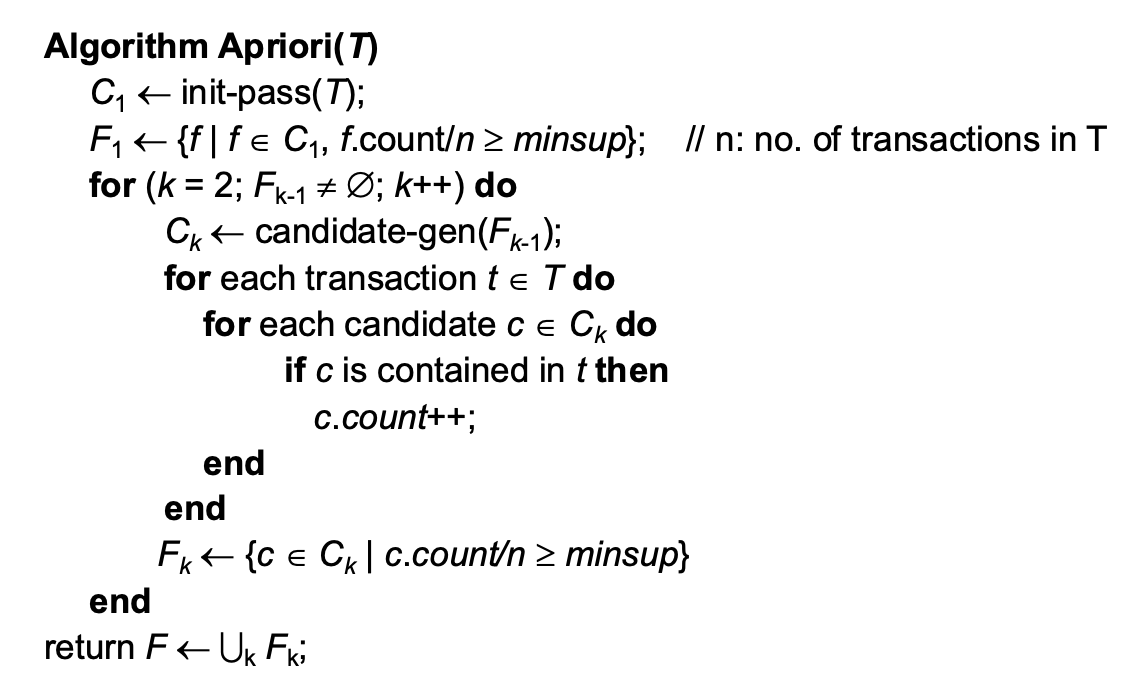
\includegraphics[width=0.8\textwidth]{Images/Apriori.png}
\end{figure}
\begin{figure}[H]
    \centering
    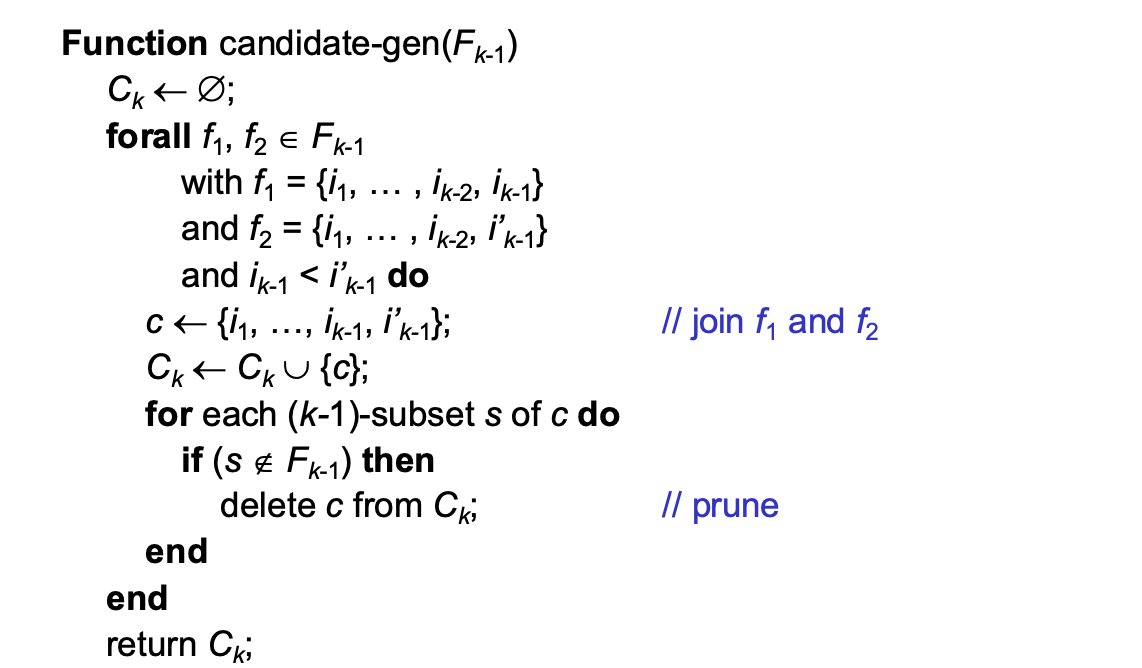
\includegraphics[width=0.8\textwidth]{Images/Candidate_gen_apriori.png}
\end{figure}

\section{MS Apriori}
sort in ascending
\begin{figure}[H]
    \centering
    \begin{minipage}[t]{0.32\textwidth}
        \centering
        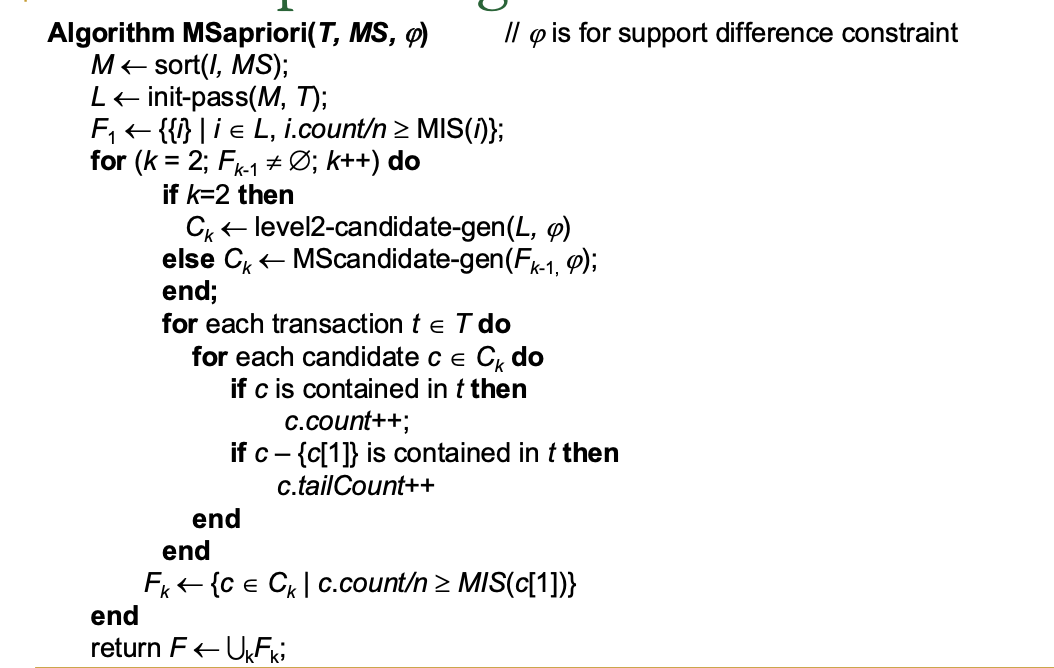
\includegraphics[width=\textwidth]{Images/MsApriori.png}
        \caption{MsApriori}
    \end{minipage}%
    \hfill
    \begin{minipage}[t]{0.32\textwidth}
        \centering
        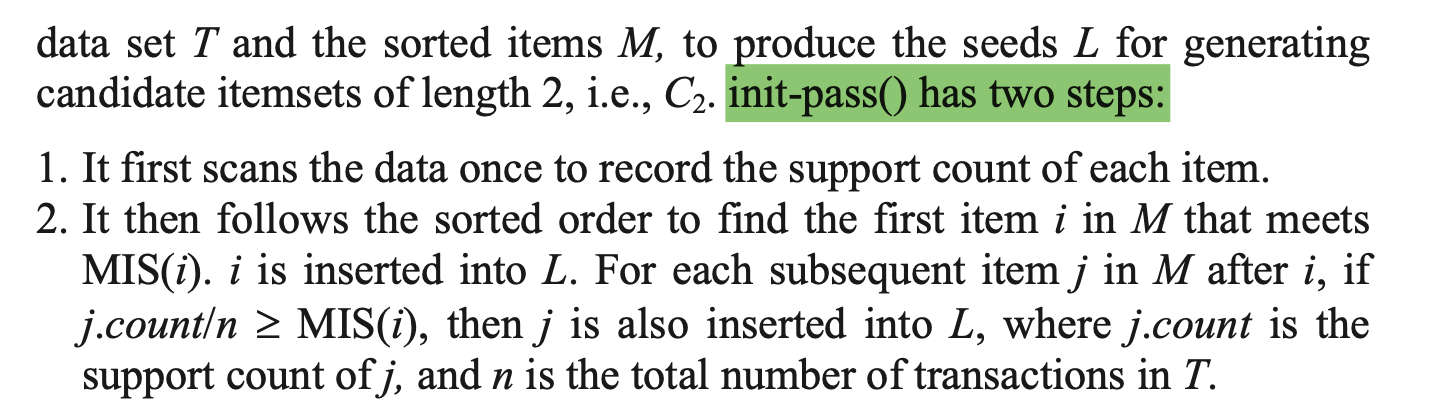
\includegraphics[width=\textwidth]{Images/init_pass.png}
        \caption{Init Pass}
    \end{minipage}%
    \hfill
    \begin{minipage}[t]{0.32\textwidth}
        \centering
        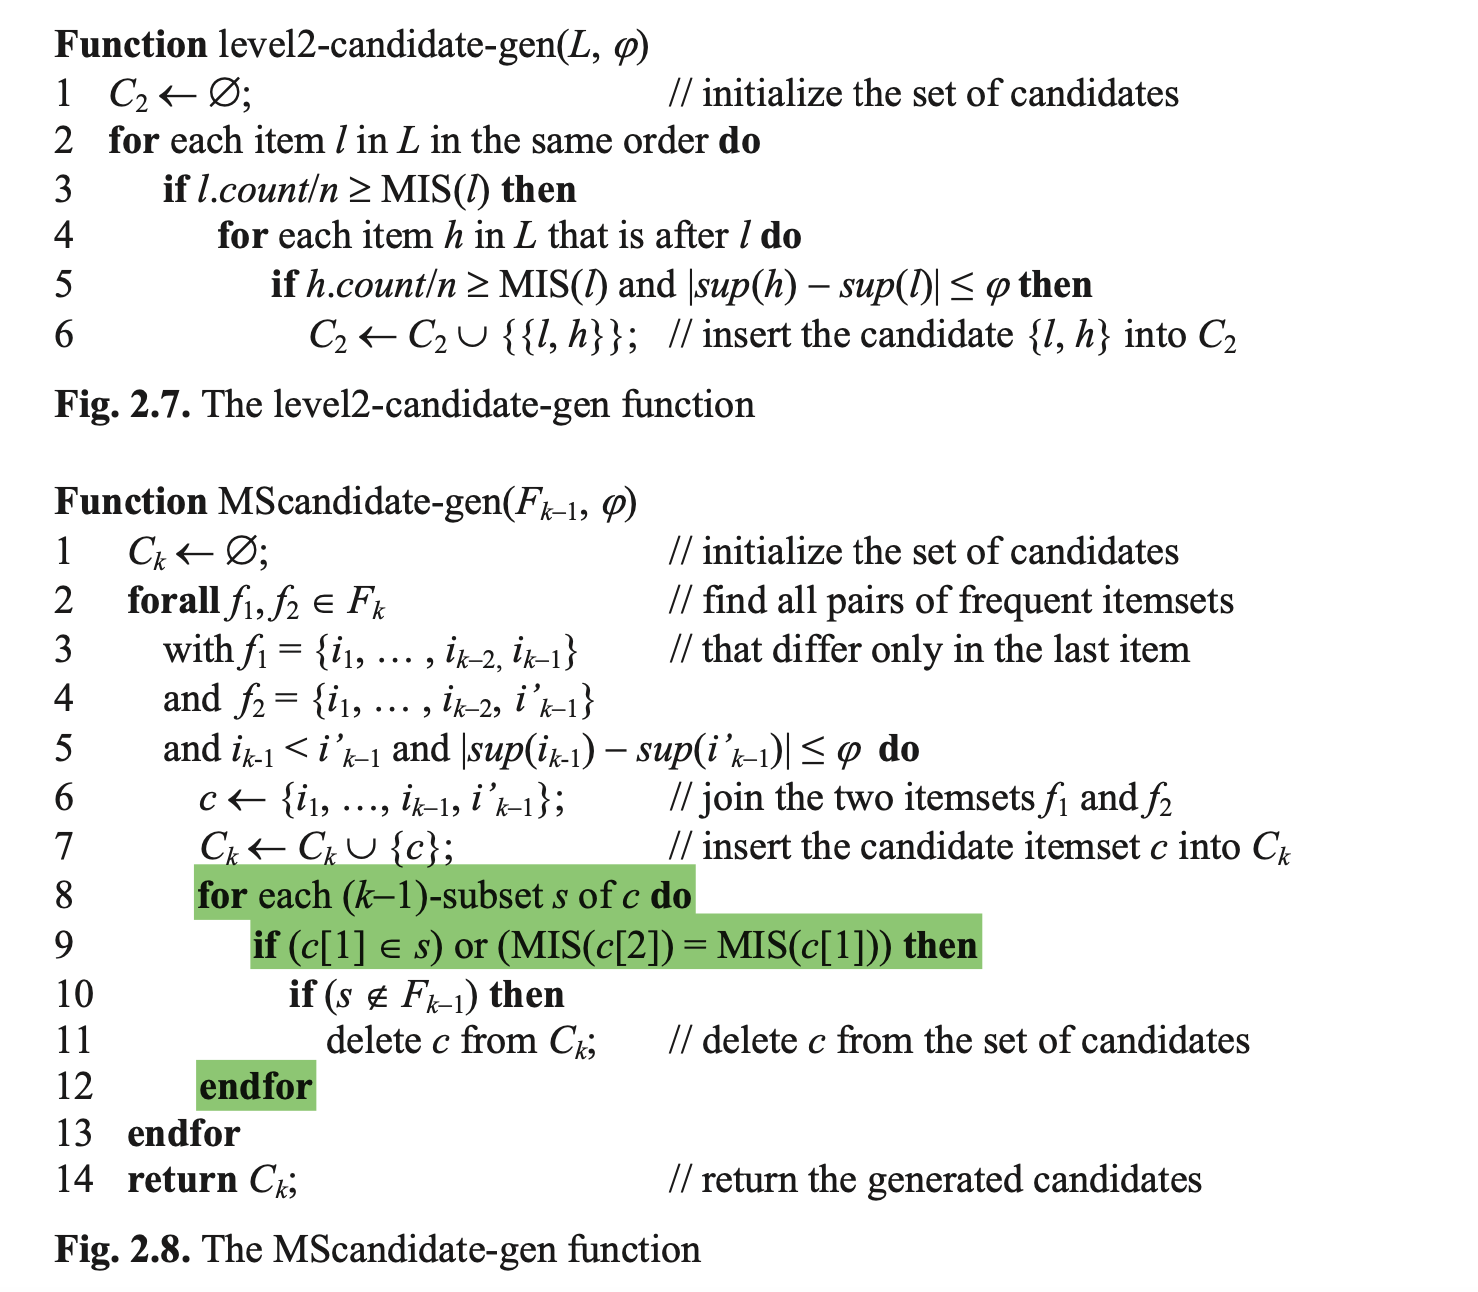
\includegraphics[width=\textwidth]{Images/Candidate_gen_MS.png}
        \caption{Candidate Gen MS}
    \end{minipage}
\end{figure}


\section{GSP (sequential pattern mining)}
\begin{figure}[H]
    \centering
    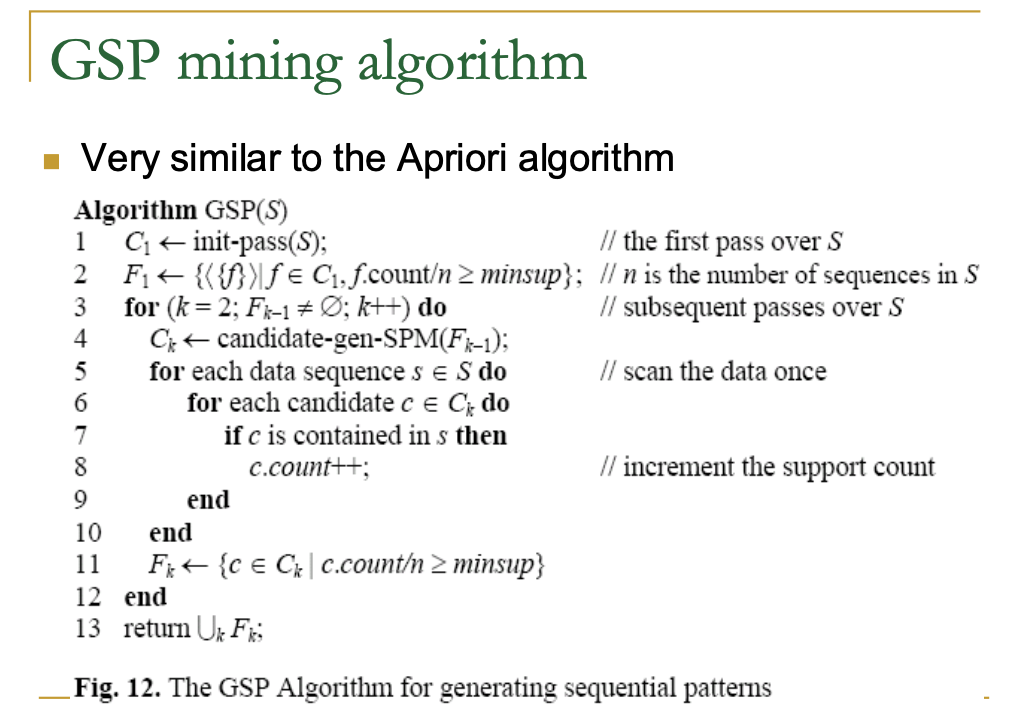
\includegraphics[width=0.8\textwidth]{Images/GSP1.png}
\end{figure}
When he says is the same as the subsequence... Means that you have to remove the parenthesis and see if the elements are in the same order.
\begin{figure}[H]
    \centering
    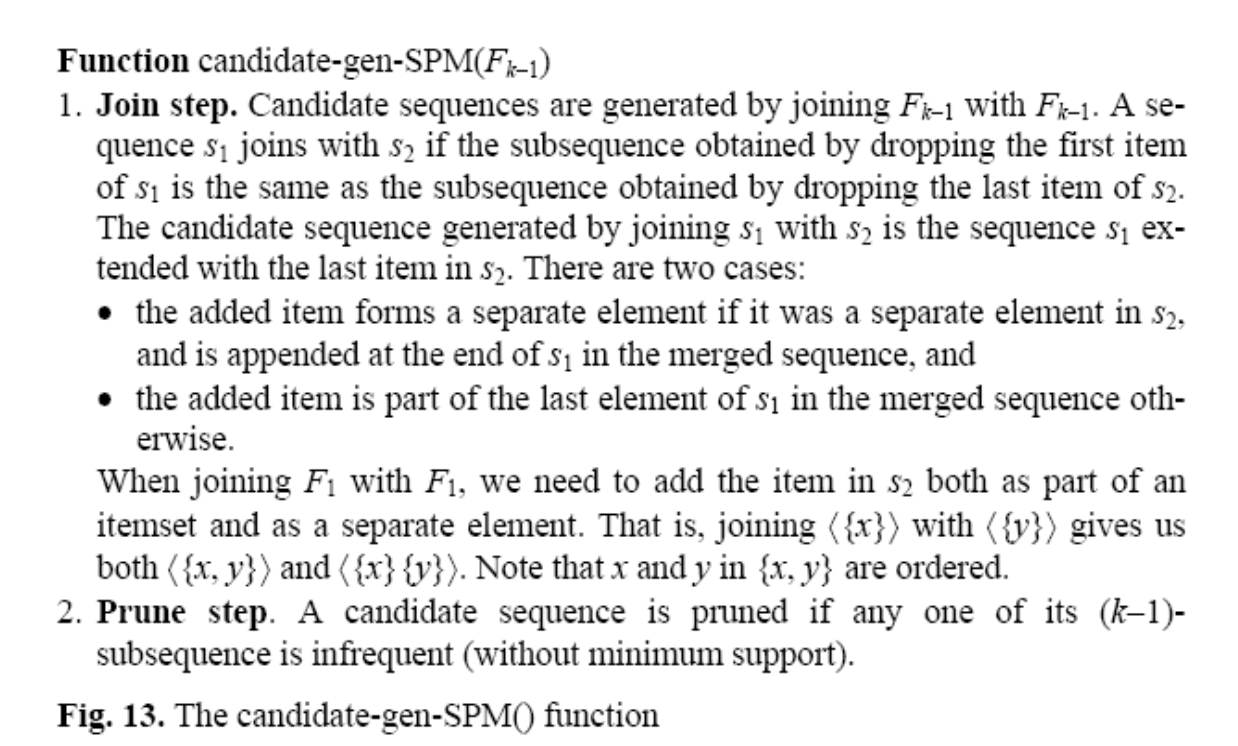
\includegraphics[width=0.8\textwidth]{Images/GSP.png}
\end{figure}

\section{Index for Classifiers}

\begin{table}[H]
    \centering
    \begin{tabular}{|l|l|}
        \hline
        \textbf{Metric}           & \textbf{Description / Formula}                                       \\ \hline
        Accuracy                  & $\frac{\text{Correctly Classified Examples}}{\text{Total Examples}}$ \\ \hline
        Precision                 & $\frac{TP}{TP + FP}$: Of predicted positives, how many are correct.  \\ \hline
        Recall/sensitivity (TPR)  & $\frac{TP}{TP + FN}$: Of actual positives, how many are identified.  \\ \hline
        $F_1$ Score               & $2 \times \frac{p \cdot r}{p + r}$: Combines precision and recall.   \\ \hline
        Specificity (TNR)         & $\frac{TN}{TN + FP}$: True negative rate.                            \\ \hline
        False Positive Rate (FPR) & $1 - \text{TNR}$                                                     \\ \hline
        ROC Curve                 & Plot: FPR (x-axis) vs. TPR (y-axis).                                 \\ \hline
    \end{tabular}
    \caption{Summary of Classification Metrics}
\end{table}


\section{Decision trees}
\begin{figure}[H]
    \centering
    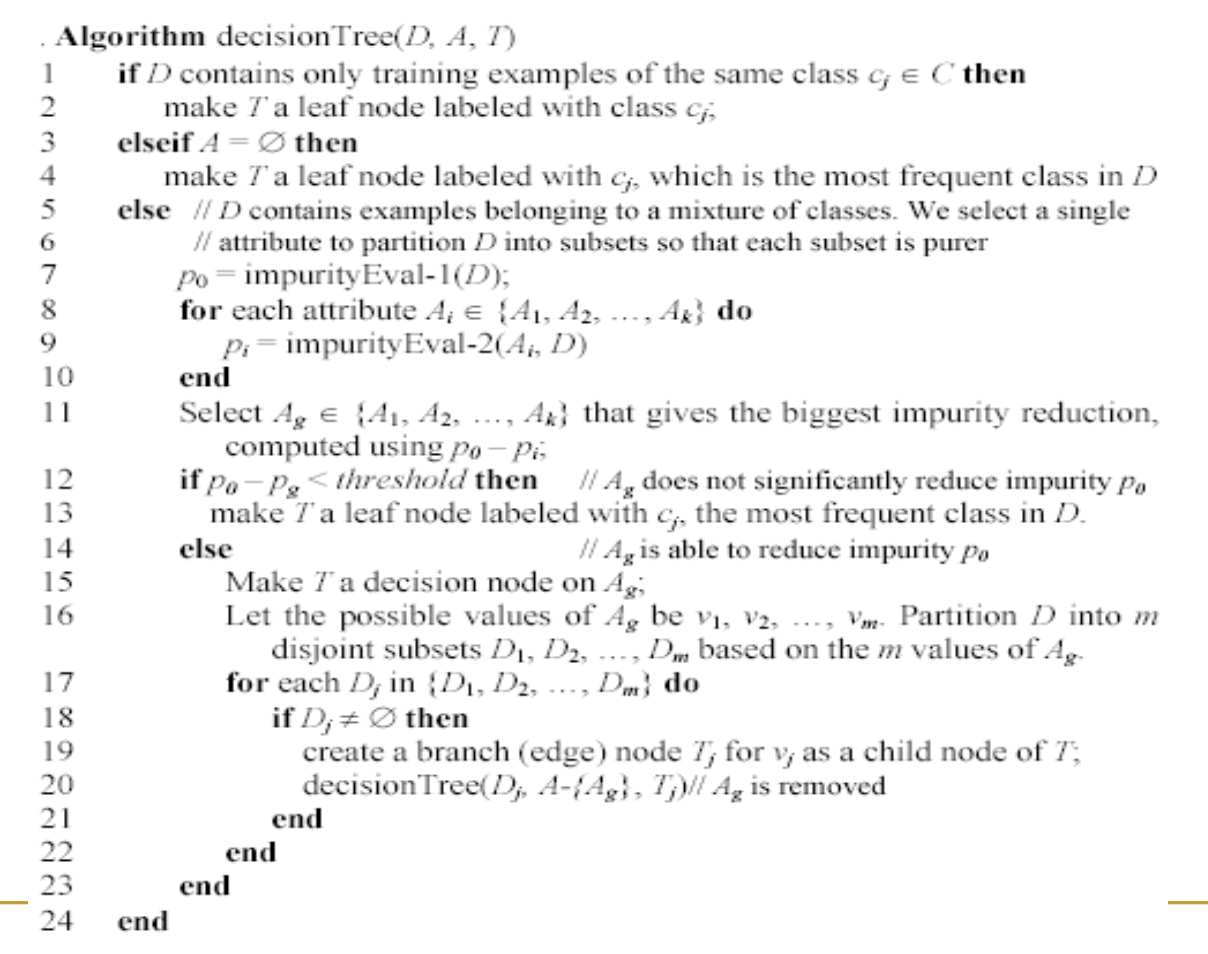
\includegraphics[width=0.8\textwidth]{Images/DecisionTree.png}
\end{figure}

\paragraph{Entropy}
D is the dataset. C are the different classes in the dataset.

\[
    \text{entropy}(D) = - \sum_{j=1}^{|C|} \text{Pr}(C_j) \log_2 \text{Pr}(C_j)
\]

Is a positive value.
The sum of the probabilities of the classes is 1.
The more the data is purer, the more the entropy value is close to zero.
Worst entropy is 1 (all the classes are equally distributed).

\[
    \text{entropy}_{A_i}(D) = \sum_{j=1}^{v} \frac{|D_j|}{|D|} \times \text{entropy}(D_j)
\]

This value is the entropy if we choose to partition the data over attribute A. There are v possible values for the attribute A.

\[
    \text{gain}(D, A_i) = \text{entropy}(D) - \text{entropy}_{A_i}(D)
\]
The higher the gain the better

\section{Naive based classification}
Product rule
\[
    \text{Pr}(a1, a2) = \text{Pr}(a1) \text{Pr}(a2 | a1)
\]
Product rule for conditional probability
\[
    \text{Pr}(a1, a2|c) = \text{Pr}(a2|c) \text{Pr}(a2 | a1, c)
\]
General case
\[
    \text{Pr}(a_1 \cdots a_n \mid c) = \text{Pr}(a_1 \mid c) \text{Pr}(a_2 \mid c, a_1) \cdots \text{Pr}(a_n \mid c, a_1 \cdots a_{n-1})
\]
Conditional independence assumption
\[
    \text{Pr}(a_i \mid c, a_1 \cdots a_{i-1}) = \text{Pr}(a_i \mid c)
\]
Goal:
\[
    \text{Pr}(c \mid (a_1 \cdots a_n)) = \frac{\text{Pr}(c)  \text{Pr}((a_1 \cdots a_n) \mid c)}{\text{Pr}(a_1 \cdots a_n)}
\]
Using the law of total probability
\[
    \text{Pr}(a_1 \cdots a_n) = \sum_{r=1}^{|C|} \text{Pr}(c) \text{Pr}((a_1  \cdots a_n) \mid c)
\]
Using the product rule and the conditional independence assumption
\[
    \text{Pr}(c \mid (a_1 \cdots a_n)) = \frac{\text{Pr}(c) \prod_{i=1}^{n} \text{Pr}(a_i \mid c)}{\sum_{r=1}^{|C|} \text{Pr}(c) \prod_{i=1}^{n} \text{Pr}(a_i \mid c)}
\]

Adjusting the probability to account for attribute values that don't occur with that class.
\begin{figure}[H]
    \centering
    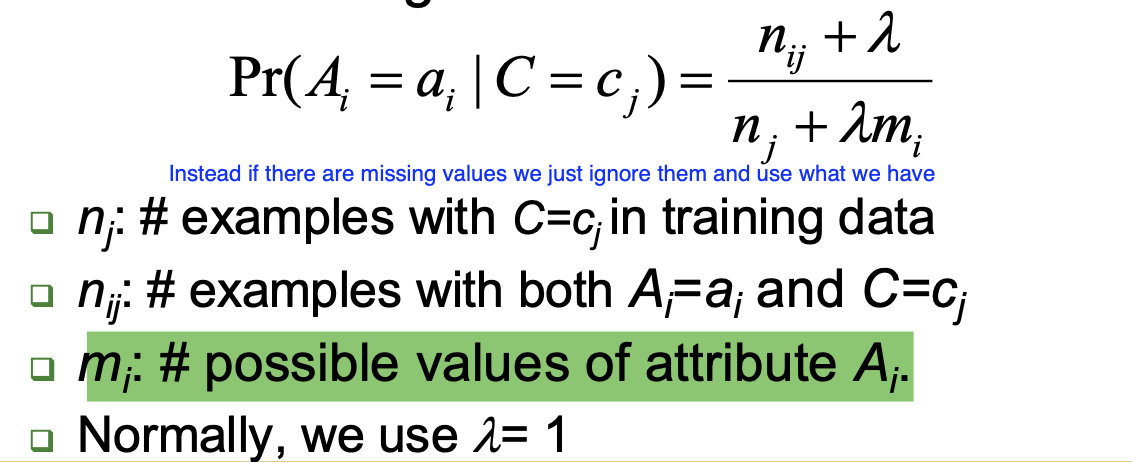
\includegraphics[width=0.8\textwidth]{Images/Zerocounts.png}
\end{figure}

\section{Naive based text classification}
\[
    \text{Pr}(c | d) = \frac{\text{Pr}(c) \text{Pr}(d|c)}{\text{Pr}(d)}
\]
\[
    = \frac{\text{Pr}(c) \prod_{k=1}^{\text{all word in d}} \text{Pr}(w_k|c)}{\sum_{r=1}^{|C|} \text{Pr}(c_r) \prod_{k=1}^{\text{all word in d}} \text{Pr}(w_k|c)}
\]
\[
    \text{Pr}(c) = \frac{\sum_{i=1}^{|D|} \text{Pr}(c|d_i)}{|D|}
\]
% This is the probability of the class c with the parameters tetha generating the document d. This depends on the probability of generating a document of length d, the possible ways of rearranging the words in the document (factorial term), the number of times the word t is in the document d and the probability of the word being generated by the class with parameters tetha.
% \[
%     \text{Pr}(d_i \mid c_j; \Theta) = \text{Pr}(|d_i|) \cdot |d_i|! \prod_{t=1}^{|V|} \frac{\text{Pr}(w_t \mid c_j; \Theta)^{N_{ti}}}{N_{ti}!}
% \]
% This is the probability of a word being generated by a class. This is at the numerator the summations on the whole set of documents of the number of times the word appears in a document multiplied per the probability of the document of being of class c.
% At the denominator we sum the same probability for all the word in the dataset.
\[
    \text{Pr}(w|c) = \frac{\sum_{i=1}^{|D|} N_{i} \text{Pr}(c|d_i)}{\sum_{s=1}^{|V|} \sum_{i=1}^{|D|} N_{si} \text{Pr}(c|d_i)}
\]

% \[
%     \text{Pr}(d_i \mid \hat{\Theta}) = \sum_{r=1}^{|C|} \text{Pr}(c_r \mid \hat{\Theta}) \text{Pr}(d_i \mid c_j; \Theta)
% \]

% \section{SVMs}
% Krun Tucker conditions

% \[
%     \frac{\partial L_p}{\partial w_j} = w_j - \sum_{i=1}^{r} y_i \alpha_i x_{i,j} = 0, \quad j = 1, 2, ..., m
% \]

% \[
%     \frac{\partial L_p}{\partial b} = - \sum_{i=1}^{r} y_i \alpha_i = 0
% \]

% \[
%     y_i \left( \langle w, x_i \rangle + b \right) \geq 1, \quad i = 1, 2, ..., r
% \]

% \[
%     \alpha_i \geq 0, \quad i = 1, 2, ..., r
% \]

% \[
%     \alpha_i \left( y_i \left( \langle w, x_i \rangle + b \right) - 1 \right) = 0, \quad i = 1, 2, ..., r
% \]

% Wolfe dual
% \[
%     L_D = \sum_{i=1}^{r} \alpha_i - \frac{1}{2} \sum_{i=1}^{r} \sum_{j=1}^{r} y_i y_j \alpha_i \alpha_j \langle x_i, x_j \rangle
% \]

% \[
%     \text{Subject to:} \quad \sum_{i=1}^{r} y_i \alpha_i = 0
% \]

% \[
%     \alpha_i \geq 0, \quad i = 1, 2, ..., r
% \]

% The linear separator
% \[
%     \langle w, x \rangle + b = \sum_{i \in SV} y_i \alpha_i \langle x_i, x \rangle + b = 0
% \]


% Soft margin
% \[
%     \frac{\partial L_p}{\partial w_j} = w_j - \sum_{i=1}^{r} y_i \alpha_i x_{i,j} = 0, \quad j = 1, 2, ..., m
% \]

% \[
%     \frac{\partial L_p}{\partial b} = - \sum_{i=1}^{r} y_i \alpha_i = 0
% \]

% \[
%     \frac{\partial L_p}{\partial \xi_i} = C - \alpha_i - \mu_i = 0, \quad i = 1, 2, ..., r
% \]

% \[
%     y_i \left( \langle w, x_i \rangle + b \right) - 1 + \xi_i \geq 0, \quad i = 1, 2, ..., r
% \]

% \[
%     \xi_i \geq 0, \quad i = 1, 2, ..., r
% \]

% \[
%     \alpha_i \geq 0, \quad i = 1, 2, ..., r
% \]

% \[
%     \mu_i \geq 0, \quad i = 1, 2, ..., r
% \]

% \[
%     \alpha_i \left( y_i \left( \langle w, x_i \rangle + b \right) - 1 + \xi_i \right) = 0, \quad i = 1, 2, ..., r
% \]

% \[
%     \mu_i \xi_i = 0, \quad i = 1, 2, ..., r
% \]

% \[
%     \text{Maximize: } L_D(\alpha) = \sum_{i=1}^{r} \alpha_i - \frac{1}{2} \sum_{i=1}^{r} \sum_{j=1}^{r} y_i y_j \alpha_i \alpha_j \langle x_i, x_j \rangle
% \]

% \[
%     \text{Subject to:} \quad \sum_{i=1}^{r} y_i \alpha_i = 0
% \]

% \[
%     0 \leq \alpha_i \leq C, \quad i = 1, 2, ..., r
% \]

% \end{multicols}
\end{document}